\chapter{Approche modulaire des réseaux de neurones}
De nombreux modèles biologiques présentent des architectures modulaires. Notre conception du monde se présente en fait sous une forme de modularité.
Présentation d'exemples de théories dérivées d'une modularité bio-inspirée. 
Brooks \cite{brooks_sumsumption_85}

Réseaux associés aux systèmes complexes, interactions

The mind, the brain and complex adaptative systems : how a mind resides in a brain (1962). Propose la near decomposability 

Trouver un questionnement, un exemple qui parle de modularité dans les systèmes biologiques:  

En tant qu'humain, nous comprenons le monde de notre point de vue, en le décomposant pour qu'il semble accessible : en effet notre raisonnement est modulaire, notre système social, groupes d'individus, etc. Nos contructions sont modulaires : programme informatique ... Il est difficile de concevoir et surtout de comprendre, en tant qu'individu un système qui ne serait pas décomposable en modules. Prenons comme exemple les réseaux de neurones profonds : la compréhension  et l'interprétabilité ces programmes est un défi de la recherche actuelle. Pour cette interprétation, on cherche des éléments symboliques, des groupes, des communautés. 
La décomposition des sciences elles même, par exemple, nous permet de trouver des solutions aux problèmes a des échelles différentes. Le programmeur n'a pas besoin de comprendre en profondeur quels transistors composent les circuits; l'expert.e en electronique n'a pas besoin de d'abord résoudre les équations qui régissent les mouvements ioniques au sein des transistors pour concevoir des circuits, etc. Seuls les principes régissant les comportement globaux d'un système commme le transistors ont besoins d'être connus pour utiliser ces sytèmes dans une tâche; tâche qui consituera également un module dans son ensemble et qui sera régie par des principes généraux, du transitor à l'utilisation d'un logiciel de dessin graphique. 
Mais est ce que cette hiéarchie modulaire est essentiellement subjective ? A priori non. Une organisation modulaire est présente et calculable dans de nombreux systèmes. 

%%%%%%%%%%%%%%%%%%%%%%%%%%%%%%%%%%%%%%%%%%%%%%%%%%%%%%%%%%%%%%%%%%%%%%%%%%%
% SECTION 1 introduction via la biologie, exemples 
%%%%%%%%%%%%%%%%%%%%%%%%%%%%%%%%%%%%%%%%%%%%%%%%%%%%%%%%%%%%%%%%%%%%%%%%%%%%
\section{La modularité, répandue dans les système biologiques}

Qui dit système complexe dit système modulaire ? (pour la fin)

\subsection{Systèmes complexes}

Les systèmes, dans leur échelles, sont donc complexes. Si on peut approximer certains systèmes pour les étudier, ils restent liés au sein d'un vaste écosystème. Ainsi, l'étude de la modularité des systèmes est présente au sein des approches biologiques.

\subsection{cerveau}

L'étude des réseaux biologiques, notamment, a fait émerger l'idée d'architectures modulaires. Et si on rajoute l'idée d'apprentissage, l'étude des cerveaux est une mine d'information et de questionnement quant aux structures et propriétés le permettant. 
Les premières propositions d'études du cerveau humain datent du début du XXeme siècle. Déjà, un découpage en aires est proposé pour expliquer le fonctionnement de cet organe, notamment avec les travaux de Broca et Wernicke qui mettent en lumière des zones du cerveau qui semblent responsable du langage. Le modèle connexioniste du cerveau, formalisé à partir de ces travaux par Geschwind dans les années 60 , décompose ainsi le langage en plusieurs fonctions : la compréhension, la lecture et l'action de parler. Ce modèle n'est plus vraiment utilisé, mais la décomposition 
Avec l'avènement des outils d'imagerie, le cerveau a pu être cartographié plus préciséement en un ensemble d'aires, agissant comme modules fonctionnels au sein d'une structure complexe; ces aires sont elles mêmes composées de modules distincts, etc. 

Le cerveau est ainsi présenté en modèle et motivation principale lorsqu'il s'agit de construire des réseaux de neurones artificiels. 
- Nombreuses études s'appuient sur le système modulaire : le cerveau \cite{primate_cortex_91,mountcastle_columnar_1997,binzegger05}


- Modularité structurelle : exemple du cortex visuel
- Connexions
- Modularité hiérarchique( modules de modules) : exemples.

%%%%%%%%%%%%%%%%%%%%%%%%%%%%%%%%%%%%%%%%%%%%%%%%%%%%%%%%%%%%%%%%%%%%%%%%%%%%%
% SECTION 2 : définitions et propriétés
%- Tour d'horizons des définitions : en bio, en ingénieurie. Auto-organisation, conséquence de la modularité ? 
%- Taxonomie : fonctionnelle, stucture modulaire,emergence 
%- Position de l'autrice du manuscrit sur la modularité, intéret des différentes modularités
%- Discussion : est ce que notre esprit modulaire veut trouver de la modularité a tout prix ? ( quand la mod est fonctionnelle, peut etre biais de nos représentations ? Mais, on observe assez objectivement des modules physiques via les connexions dans de nombreux réseaux. Evolution l'a fait comme ca, probablement une réponse globale a un problème. 
%- Echelles de la modularité. 
%- Activation d'autres modules
%- Mutli-modalité - un mot, rappel dans une autre partie
%%%%%%%%%%%%%%%%%%%%%%%%%%%%%%%%%%%%%%%%%%%%%%%%%%%%%%%%%%%%%%%%%%%%%%%%%%%%%%%

\section{Quelle définition de la modularité ?}

Il s'agit de tirer une définition claire de ce qu'on appelle modularité. Entre l'étude des systèmes biologiques et l'ingénieurie des réseaux de neurones, l'aspect modulaire des réseaux et plus généralement des systèmes peut se définir de plusieurs manières. 

\subsection{Modularité structurelle}

Lorsque le système possède une structure définie de réseau, typiquement un réseau de neurones, on peut définir une modularité en terme de graphe.

\subsubsection{Réseaux en "petit-monde"}
Definition: type de graphe dans lequel la distance moyenne entre deux noeuds est proportionnelle à log(N), N le nombre de noeuds. C'est à dire, un graphe dans lequel on trouvera un chemin assez court entre n'importe quels noeuds. 
Particularités : forme souvent des cliques ( sous graphes fortement connexes), donc une structure modulaire. Par contre, tous les réseaux small world ne sont pas necessairement modulaire. 
Souvent admis que le cerveau en tant que réseau de neurones est small world. 

\begin{figure}
\begin{minipage}{0.5\textwidth}
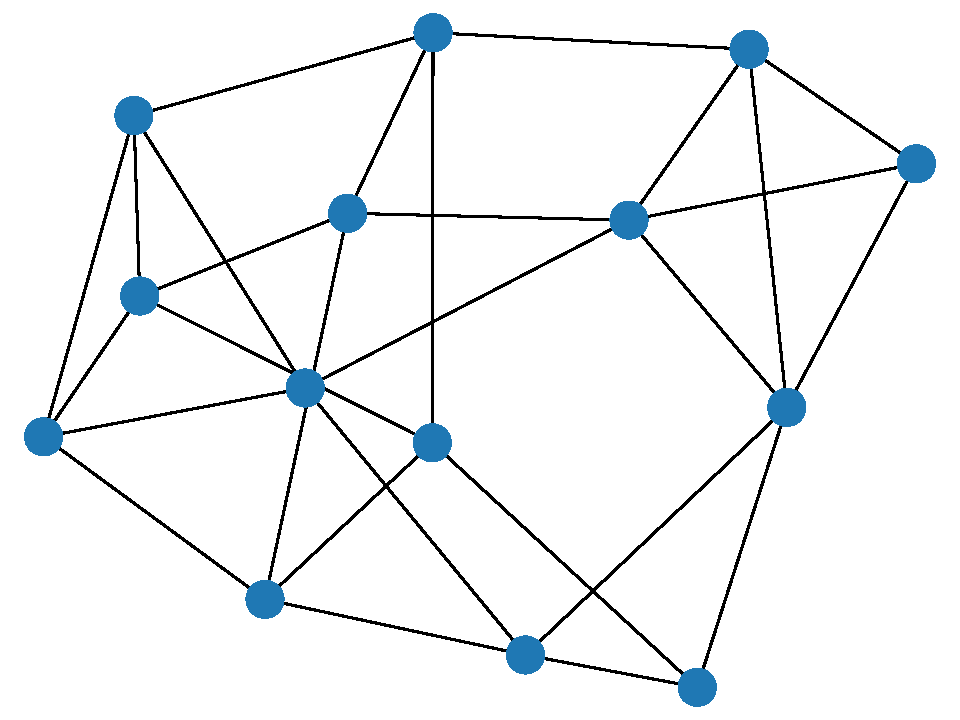
\includegraphics[width=\textwidth]{watts_strogatz.pdf}
\caption{Réseau aléatoire "petit-monde" créé avec l'algorithme de Watts-Strogatz}
\end{minipage}
\begin{minipage}{0.5\textwidth}
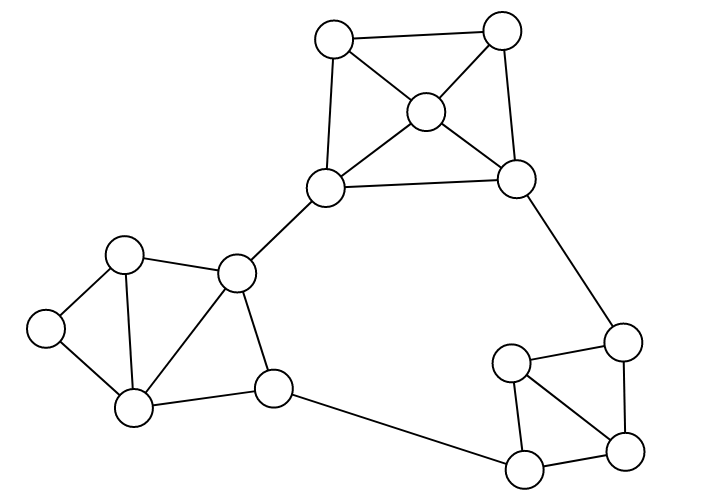
\includegraphics[width=\textwidth]{small_world_net.png}
\caption{Réseau modulaire : il possède une propriété de "petit monde" mais des modules, zones fortement connectées, sont identifiables.}
\end{minipage}

\end{figure}
\subsubsection{Modularité auto-similaire}

Exemples ?? \cite{Meunier2010ModularAH}
Modularité hiérarchique présente l'avantage de maintenir une activité dans le réseau sans que ca ne colonise tout ni ne s'eteigne, ce qui est nécessaire pour la computation. 


\subsubsection{Mesure la modularité}

clustering coefficient
proximity ratio
scale free networks

\subsubsection{Def}
\cite{Hilgetag2015IsTB} : différencie réseaux small world et réseaux hiararchique modulaires, et statue qu'un réseau peut etre "hiérarchique modulaire" même s'il n'est pas small world, mais possède une dimension topologique finie. 
\cite{Meunier2010ModularAH} : statue que un réseau modulaire est small world,

\subsection{Modularité fonctionnelle}


\subsection{Modularité temporelle}

La modularité s'associe aux séquences dans le cerveau. On peut donc raisonnablement définir 


%%%%%%%%%%%%%%%%%%%%%%%%%%%%%%%%%%%%%%%%%%%%%%%%%%%%%%%%%%%%%%%%%%%%%%%%%%%%%%%%%%%%%%%%%%%%%%%%%%%%%%%%%%%%%%%%%%%%%%%%%%%%%%%%%%%%%%%%
% SECTION 3: quel intéret à utiliser des architectures modulaires pour l'apprentissage ? 
% - 
%%%%%%%%%%%%%%%%%%%%%%%%%%%%%%%%%%%%%%%%%%%%%%%%%%%%%%%%%%%%%%%%%%%%%%%%%%%%%%%%%%%%%%%%%%%%%%%%%%%%%%%%%%%%%%%%%%%

\section{Intérêt computationnel des réseaux modulaires}

Barabasi : Hypothèse que les réseaux small world présentent un avantage evolutionnaire.

\subsubsection{réponse a un problème de contrainte physiques, énergétiques}

- Parallelisme, calcul et small world networks : réponse a un problème de contrainte physiques, énergétiques. 
- Calcul distribué 
- Automates cellulaires  ?


\subsection{Types de connexions}

Opaque vs tout savoir


\subsection{Modularité et émergence d'un apprentissage ? }

La modularité est liée a la complexité des systèmes, donc l'emergence de comportements chaotiques et/ou synchronisés. 
SYSTEMATIC GENERALIZATION : WHAT IS REQUIRED
AND CAN IT BE LEARNED ? : 
Our findings show that the generalization of modular models is much more systematic and that it is highly sensitive to the module layout, i.e. to how exactly the modules are connected.

%%%%%%%%%%%%%%%%%%%%%%%%%%%%%%%%%%%%%%%%%%%%%%%%%%%%%%%%%%%%%%%%%%%%%%%%%%%
% SECTION 4 En pratique, ou en est on des réseaux de neurones modulaires ?
%%%%%%%%%%%%%%%%%%%%%%%%%%%%%%%%%%%%%%%%%%%%%%%%%%%%%%%%%%%%%%%%%%%%%%%%%%%%%ùù

\section{Réseaux de neurones modulaires}

- Challenges et intérêt potentiel des réseaux de neurones modulaires ? -> Evolution (wertmer, meunier) : pousser plus loin pour etre au jus sur les challenges actuels ( voir du coté du deep : quelles sont les motivations et les challenges ? 


\subsection{Deep Learning}
Grosse boite noire qui ont des performances remarquables sur le traitement des images, du langage etc; leur représentation est toujours un challenge.
- Réseaux qui apprennent a s'organiser en modules. Interet. Limites ? Performances ? \cite{Andreas2016NeuralMN,Kirsch2018ModularNL}
"The NMN approach is intuitively appealing but its
widespread adoption has been hindered by the large amount of domain knowledge that is required
to decide (Andreas et al., 2016) or predict (Johnson et al., 2017; Hu et al., 2017) how the modules
should be created (parametrization) and how they should be connected (layout) based on a natural
language utterance. Besides, their performance has often been matched by more traditional neural
models" ( systematic generalization article ) 
- Trouver des modules dans les réseaux pour les expliquer ? \cite{Watanabe2018ModularRO,Csordas2021AreNN}
are neural net modular : "it uses different modules for very different functions = Pspecialize," et "it uses the same module for identical functions that
may have to be performed multiple times = Preuse"
- Reconciling deep learning with symbolic artificial intelligence: representing objects and relations(2019)
Pb du deep learning = Data inefficiency (comparé a l'humain);Poor generalisation; Lack of interpretability.

\subsection{Réseaux auto-organisés}

Plus qu'en deep learning, les réseaux de neurones auto-organisés
- Auto-organisation prend une profonde inspiration biologique, tout comme les modules.
- Exemple de réseaux auto-organisés modulaires : développer dans la partie suivante.

\cite{johnsson_associative_2009}
\cite{LampinenClusteringPO}
\cite{parisiLL}

\subsection{Construire une architecture modulaire}


A mettre dedans : 

- Réseaux top down / modulaires ? définition, a quel point un réseau est modulaire, qu'est ce qu'on appelle réseau modulaire ? 
Fonction définies au préalable vs émergence des fonctions. 
Modules définis au préalable vs émergence des modules. 


%%%%%%%%%%%%%%%%%%%%%%%%%%%%%%%%%%%%%%%%%%%%%%%%%%%%%%%%%%%%%%%%%%%%%%%%%%%%%%%%
% SECTION 5 : proposer des enjeux par rapports au réseaux listés précedemment 
%%%%%%%%%%%%%%%%%%%%%%%%%%%%%%%%%%%%%%%%%%%%%%%%%%%%%%%%%%%%%%%%%%%%%%%%%%%%%%%%


\section{Enjeux d'une architecture modulaire de SOMs}

On connait plutot bien les SOM, mais on sait que des comportements nouveaux peuvent émerger lorsqu'on met en interaction des systèmes étudiés séparément. 
On peut donc se poser la question des comportements qui peuvent survenir dans ce cas.

Dans les structures de cartes étudiés, modularité forte dans le sens ou les fonctions des modules sont prédéfinies. Si on ne fournit que les règles d"interaction, ou est ce qu'on se situe ? 
 
%%%%%%%%%%%%%%%%%%%%%%%%%%%%%%%%%%%%%%%%

Plan de la partie ! 

 

\begin{enumerate}
\item Intro : Notre monde est modulaire, en tout cas nous l'interprétons en tant que tel. Proposé déjà dans les années 60 - breve histoire des réseaux de neurones ?
Remarquer que nous, observeur, raisonne et se construit modualairement. Il nous est difficile de concevoir les choses autrement. 
Les disciplines sientifiques par ex, un domaine obéit a des principes
\item Qu'appelle t-on la modularité ? Définitions claires et propriétés
	\begin{itemize}

		\item Definition
			\begin{enumerate}
			\item Structurelle, dans les systèmes réseaux
			\item Fonctionnelle, dans les systèmes dont on ne connait pas la structure ?\\
			\item Temporelle / mais est ce que le temps ce n'est qu'une dim de plus
			\item Modularité hiérarchique attention : deux defs a hiérarchiques. Soit c'est une histoire de connexions, soit d'auto-similarité. On parle nous de l'auto similarité !!! Au contraire l'autre forme de hiérarchie n'est pas observée en bio.
			\end{enumerate}
		
		\item Propriétés de la modularité 
			\begin{enumerate}
			\item Auto-organisation
			\item Types de connexions
			\item Emergence
			\end{enumerate}
	\end{itemize}	
\item Exemples Biologiques et computationnels
	\begin{enumerate}
	\item Biologie : opti evolution a priori...
	\item Computationnel : pareil.
	\end{enumerate}
	
\item Maintenant qu'on sait ce que sont les systèmes modulaires, en quoi on peut faire de l'apprentissage avec ? Quels sont les intérêts ?
	\begin{enumerate}
		\item Exemples de réseaux auto-organisés
		\item Exemples de réseaux de neurones : deep learning
	\end{enumerate}

\end{enumerate}





